\documentclass{article}
\usepackage{graphicx}

\title{Exposure and childhood diagnoses: a toy example}
\author{Your Name}

\begin{document}
\maketitle

% One sentence per line: git diffs then show exactly which sentence changed.

\section{Methods}
We used a simulated cohort of 20\,000 individuals born 1990--2010.
For each of eight diagnoses, we fitted a logistic regression of the diagnosis on exposure, adjusting for sex.
Analyses were run on a secure server, and only aggregate results were exported.
Cells with fewer than five cases were suppressed before export.

\section{Results}
Exposure was associated with higher odds of asthma, ADHD and obesity (Figure~\ref{fig:main}).
There was little evidence of association with anxiety or hypertension.

\begin{figure}
  \centering
  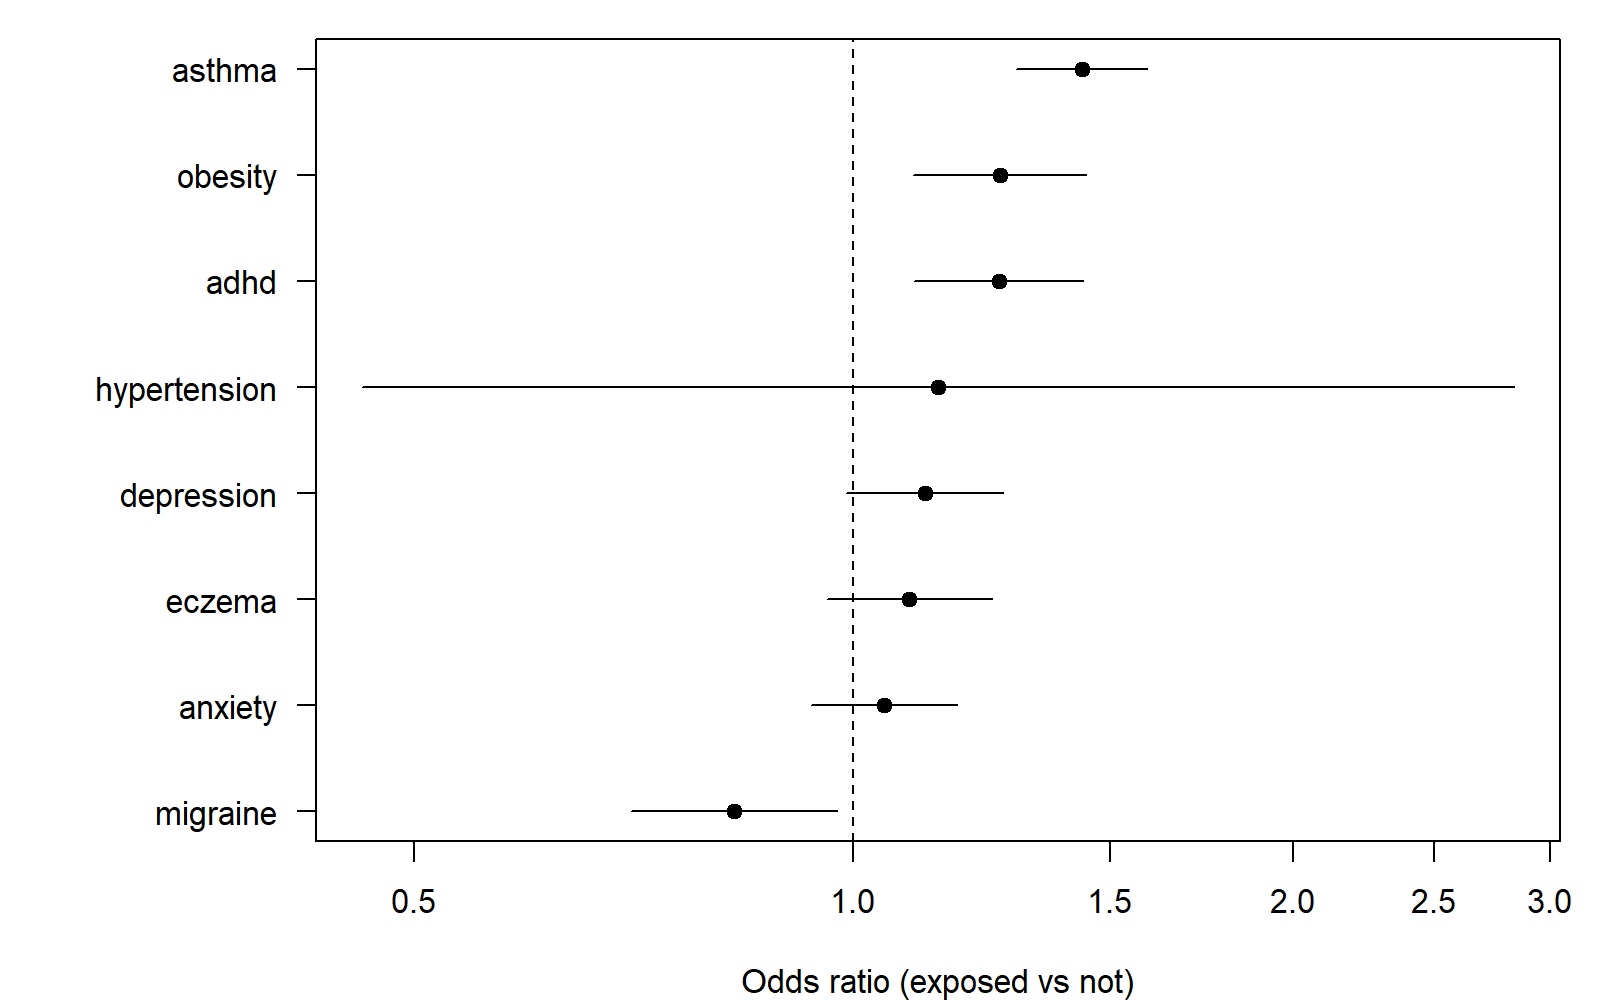
\includegraphics[width=\textwidth]{../results/figure_main.png}
  \caption{Odds ratios with 95\% confidence intervals.}
  \label{fig:main}
\end{figure}

\end{document}
